\documentclass[letterpaper,11pt]{article}

%=================Begin:Packages===================

\usepackage[utf8]{inputenc}
\usepackage{a4wide}
\usepackage[english]{babel}
\usepackage{scalerel}
\usepackage{hyperref}
\usepackage{amsmath,amsfonts,amsthm} % amssymb
\usepackage{enumitem}
\usepackage{harpoon}
\usepackage[normalem]{ulem}
\usepackage{xargs}                      % Use more than one optional parameter in a new commands
\usepackage[pdftex,dvipsnames]{xcolor}  % Coloured text etc.

%=================End:Packages===================

%==================Begin:Style===================

\newtheorem{definition}{Definition}
\newtheorem{theorem}{Theorem}
\newtheorem{lemma}{Lemma}


\newcommandx{\handan}[2]{{\uline{#1}}\textcolor{red}{(#2)}}
%\newcommandx{\handan}[2]{{#1}{}}
\newcommand\mathperiod{.}
\newcommand\mathcomma{,}

%===================End:Style====================

%==================Begin:Macros==================

\newcommand{\floor}[1]{\left\lfloor #1 \right\rfloor}
\newcommand{\ceil}[1]{\left\lceil #1 \right\rceil}

\newcommand{\vect}[1]{\overrightharp{\ensuremath{#1}}} % {\overset{\rightharpoonup}{#1}}

% probability with square brackets of the right size
% \newcommand{\Pr}{\ensuremath{\mathsf{Pr}}} %probability
% \newcommand{\Prb}[1]{\ensuremath{\Pr\left [#1 \right ]}}

\newcommand*\set[1]{\{ #1 \}} % in text, we don't want {} to grow
\newcommand*\Set[1]{\left\{ #1 \right\}}
\newcommand*\setst[2]{\{ #1 | #2 \}}
\newcommand*\Setst[2]%
        {\left\{\,#1\vphantom{#2} \;\right|\left. #2 \vphantom{#1}\,\right\}}

\newcommand*\List[1]{\left[ #1 \right]}  % cute abbreviations
\newcommand*\listst[2]{[ #1 | #2 ]}
\newcommand*\Listst[2]%
        {\left[\,#1\vphantom{#2} \;\right|\left. #2 \vphantom{#1}\,\right]}

% uniform random selection from set
\newcommand{\randsel}[0]{\ensuremath{\xleftarrow{\text{\$}}}}

% oracles
\newcommand{\ora}[1]{\ensuremath{\mathcal{O}\mathsf{#1}}}
% oracle set
\newcommand{\oraSet}[1]{\ensuremath{\mathcal{O}\textsc{#1}}}
% algorithm
\newcommand{\algo}[1]{\ensuremath{\mathsf{#1}}}
% party
\newcommand{\prt}[1]{\ensuremath{\mathcal{#1}}}
% long-form variable
\newcommand{\var}[1]{\ensuremath{\mathit{#1}}}

%=================End:Macros=====================

%=================Begin:Definitions===================

\newcommand{\VRF}{\algo{VRF}} 
\newcommand{\RingVRF}{\algo{RingVRF}} 
\newcommand{\Sign}{\algo{Sign}} 
\newcommand{\Verify}{\algo{Verify}} 
\newcommand{\KeyGen}{\algo{KeyGen}} 
\newcommand{\Out}{\algo{Out}} 

\newcommand{\sk}{\ensuremath{\mathsf{sk}}} %secret key
\newcommand{\pk}{\ensuremath{\mathsf{pk}}} %public key
\newcommand{\verify}{\ensuremath{\mathsf{Verify}}}
\newcommand{\prove}{\ensuremath{\mathsf{Prove}}}

\newcommand{\vals}{\ensuremath{\mathcal{V}}}
\newcommand{\nvals}{\ensuremath{n}}
\newcommand{\para}{\ensuremath{\rho}}

\newcommand{\pieces}{\ensuremath{\mathcal{D}}}
\newcommand{\prepieces}{\ensuremath{\pieces'}}
\newcommand\merkleroot{\ensuremath{\mathfrak{m}}} % {\mathtt{root}}}  maybe?
\newcommand\reciept{\ensuremath{\mathfrak{C}}}

\newcommand{\val}{\ensuremath{v}}

% \newcommand{\pv}{\ensuremath{\mathcal{P}V}}

\newcommand\grace{\ensuremath{\mathsf{agp}}}

\newcommand{\encode}{\ensuremath{\mathsf{Encode}}}
\newcommand{\decode}{\ensuremath{\mathsf{Decode}}}
% \newcommand{\divi}{\ensuremath{\mathsf{Divide}}}
% \newcommand{\recons}{\ensuremath{\mathsf{Reconstruct}}}

\newcommand{\blobB}{\ensuremath{\bar{B}}} %blob
% \newcommand{\bh}{\ensuremath{B_{head}}} %block header
% \newcommand{\mprf}{\ensuremath{\pi^{mt}}} %merkle proof


\newcommand{\npvals}{\ensuremath{\ell_0}} % number of parachaim validators
\newcommand\primarychecks{\ensuremath{\ell_1}} 
\newcommand\secondarychecks{\ensuremath{\ell_2}} 
\newcommand\totalchecks{\ensuremath{\ell_t}} %total number of validity check
\newcommand\equivocationchecks{\ensuremath{\ell_{\mathrm{eqiv}}}}

\newcommand\basesecondarychecks{\ensuremath{\ell_b}} 
\newcommand\rfuv{\ensuremath{\ell_v}} % report factor for unavailability from validators
\newcommand{\runav}{\ensuremath{\ell_a}}
\newcommand{\rinv}{\ensuremath{\ell_f}}

\newcommand\cc{\ensuremath{\mathbin{\|}}}

% \def\newalgo#1{%
% \expandafter\newcommand\csname #1\endcsname{\mathbf{#1}}%
% }
\newcounter{symbols}
\def\newsymbol#1{%
\expandafter\newcommand\csname #1\endcsname{\hyperref[symbols:#1]\mathsf{#1}}%
\refstepcounter{symbols}\label{symbols:#1}\mathsf{#1}%
}


\title{Availability and Validity}


\begin{document}
\date{}
\maketitle


% \section{Introduction sectrions should never be numbered unless journal style demands}

...


TODO: Into giving main idea
...
We require that approval validity checks complete before finality.  We cannot however require that all validator checks conclude before finality, or even ask fishermen to begin checks before finality, so invalidity can be detected after finality.
...

...

In \S\ref{sec:parachains}, we first recall our tools like verifiable random functions, erasure coding, and state witnesses, and then describe the sharding problem and introduce our security definitions. 

We describe and instantiate our {\em availability and validity protocol} for efficient sharding as several phases across \S\ref{sec:availability_n_backing}, \S\ref{sec:approval}, and \S\ref{sec:...}.  As a rough outline,
\begin{itemize}
\item a parachain phase in which collators produce candidate parachain blocks (\S\ref{sec:parachain}) and parachain validators perform preliminary backing validity checks (\S\ref{sec:backing}),
\item a relay chain submission phase that distributes candidate parachain blocks and produces relay chain blocks (\S\ref{sec:backing} and \S\ref{sec:topology}),
\item availability (\S\ref{sec:availability}) and unavailability (\S\ref{sec:unavailability}) subprotocols that enforce availability in GRANDPA and BABE respectively,
\item assigning secondary checkers (\ref{sec:assignment}) who fuller approval validity checks (\S\ref{sec:approcal_checks}), and
\item invokation of a Byzantine fault tolerant ``finality gadget'' that gives us finality (\S\ref{sec:finality}).
\end{itemize}
We depend upon slashing to provide economic security guarantees, so we discuss slashing both in \S\ref{\sec:slashing} and when relavant in the main protocol description.

We also discuss objection procedures for fishermen in \S\ref{sec:fishermen} and collators in \S\ref{sec:collators}.



\section{Heterogeneous sharding}
% \label{sec:parachains} % sharding

We shall describe a blockchain sharding scheme through which a single beacon or {\em relay chain} can validate numerous heterogeneous shard chains.  We aim for true shared security, minimal latency, good liveness, and relative efficiency in terms of computation, network, and storage.  We refer to our shard chains by the term {\em parachains} because shard alone connotes a non-heterogeneous approach.  There exist other terms for heterogeneous approaches too, but they all connote bridged designs without shared security.

\subsection{VRFs}

A {\em verifiable random function (VRF)} is a cryptographic function that generates a pseudo-random output number from a given a secret key $\sk$ and an input string $\alpha$ called a seed, and produces a proof of correctness for the output.  In a sence, VRFs resemble a public-key analog of a cryptographic hash function with a distinguished key, such as MACs that acts as PRFs, in that a keyed hash function requires the key be shared for verification. 

Anyone with the input and the corresponding public key $\pk$ can verify the correctness of the VRF output, so VRFs should satisfy appropriate signature scheme security definitions, like EUF-CMA.  We implement output as function applied to the signature and message that must satisfy {\em uniqueness} in that each public key and message admits only one output, {\em unpredictability} for anyone without the secret key, and {\em pseduo-randomness} even for the secret key holder.

We refer readers to \cite[\S1]{Sassafras} for more formal definitions.
Almost all proof-of-stake and sharded blockchain proposals make heavy usage of VRFs.

\subsection{Chains}
% \paragraph{Relay chain:}

We expect that our sharded blockchain employs a Byzantine fault tolerant ``finality gadget'' for the relay chain that establishes agreement on finality for all shards or parachains too, like in the Polkadot and Ethereum 2.0 designs.  We let $\vals$ denote the full validator list for the relay chain, and set $\nvals := |\vals|$, which we term just validators since the relay chain remains clear from context.  We expect here that validators act as block producers for the relay chain.  

As part of our security model, we assume that $\nvals \ge 3 f + 1$ where $f$ bounds the number of validators controlled by any adversary.

% \begin{assumption}
An adversary who controls some $f' \le f$ of the $n$ (relay chain) validators knows the upcoming block producer for its own upcoming block production slots of course, but we assume Bernoulli trials with probability \handan{${f' (n-f') \over n^2}$}{I think it is not correct for BABE since there are also empty slots. Do you talk about HABE here? But even for HABE it seems not correct to me since adv knows whether it is honest slot or not with prob. 1 in HABE} describe whether they know the honest block producer assigned to individual upcoming block production slots.  In particular if ${f \over n} < {1\over3}$ then they know less than \handan{${5 \over 9}$ths}{isn't it 2/9} of the upcoming honest block producers.
% \end{assumption}
We choose this assumption because it supports overall \handan{stronger}{in which sense it is stronger?} block production mechanisms than proof-of-work or \cite{Praos}, although those would admit a better bound here. \handan{}{is this paragraph necessary for AnV scheme? I could not see the relation between knowing whether honest or adv slot and AnV scheme. It looks confusing. }

As in other finality gadget designs, the relay chain and each parachain $\para$ has its own block production protocol run within its own infrastructure.  We employ the simplifying assumption that the block producer list equals the validator list $\vals$.  

% \paragraph{Parachains:}

A parachain $\para$ refers to its block producers as {\em collators}, which could come from $\vals$ or elsewhere.  We let $\vals_\para \subset \vals$ denote the sublist of validators assigned to parachain $\para$, which we term the {\em parachain validators} of $\para$.  We also need a bound $\npvals$ such that $|\vals_\para| \ge \npvals$.

TODO: Define many methods and paramaters of parachains $\para$

In fact, we always have an epoch parameter $t$ associated to $\para$, but we subsume $t$ into $\para$ here for convenience.  Aside from time, we similarly assume the relay chain provides some randomness $r$ associated to each epoch $t$, which we similarly subsume into our $\para$ notation for convenience.

We prefer if subscripts always denote higher level properties, like identifying parachains, cryptographic keys, etc.  We favor indexing bracket notation like $\vals[i] = \vals_\para[j]$ when identifying individual list elements, as index notation simplifies definitions and avoids mixed role subscripts. 

\subsection{Blocks}

We normally prevent blocks from referencing data in other blocks directly, e.g. UTXOs, because doing so incurs unacceptable storage overhead.  Instead, all blockchains have some associated state for which blocks describe a state transition, normally stored as a Merkle tree so that the Merkle root acts as a commitment to the entire state.  As a brutal convenience, we further subsume any current state commitments into our $\para$ notation.  We let $\hat{\para}$ denote the parachain state $\para$ but with full attached state required by collators, not just the state commitments. 
% TODO: Expand \para into immutabel \para mutable \hat{para} with the commitments 

Consider a block $B$.  We distinguish a header $B_{\mathsf{head}}$ and body $B_{\mathsf{body}}$ of a block $B = (B_{\mathsf{head}},B_{\mathsf{body}})$.  We ask that $B_{\mathsf{head}}$ contain $H(B_{\mathsf{body}})$ and commitments to the associated state before and after running $B$, normally Merkle roots.  

In principle, any block might incorporate additional associated data $M$ also referenced by $B_{\mathsf{head}}$.  We shall not belabour the associated data $M$ here, so anyone who requires it should read thoughtfully.

\begin{definition}\label{def:pob}
We define a {\em state witness procedure} to consists of
\begin{itemize}

\item a randomized algorithm $\prove_{\hat{\para}}$ that executes a block $B$, and maybe $M$, and returns a witness proof $\pi_B$ of any transitions to the associated state, as well as 
\item deterministic algorithms $\verify_\para$ and $\verify_{\hat{\para}}$ that take the blob $\blobB = (B,\pi_B,M)$ execute $B$ applying the state transition to either the commitments in $\para$ or the full state in $\hat{\para}$, and returns $\mathsf{true}$ and mutates $\para$ or $\hat{\para}$, if and only if $B$ executes correctly with the state transition given by the witness $\pi_B$. 
\end{itemize}
\end{definition}
We disallow $\prove_{\hat{\para}}$ from modifying the associated state commitments in $\para$ and only permit $\verify_{\hat{\para}}$ to do so when returning $\mathsf{true}$.  We note that $\verify_\para$ and $\verify_{\hat{\para}}$ make $B$ the more recent block of $\para$, so they should normally fail if $B$ already exists in $\para$ under most chain designs. 

As a convenient Merkle tree notation, we let the notation $\vect{xz}$ denote the copath witness proving that $z$ is a leaf of a Merkle tree with root $x$.  We support internal nodes in this notation too, so $\vect{xz} = \vect{xy} \vect{yz}$ if $y$ lies on the path from $x$ to $z$.  We write $B[\vect{xy}]$ to specify $B$ as the underlying Merkle tree, when not clear from context, especially when $B$ itself is a block.  We shall always write just $\vect{xy}$ when $x$ and $y$ lie in the state tree associated to some blockchain.  

\newcommand\rin{\ensuremath{r_{\mathsf{in}}}} % {\ensuremath{r_0}}
\newcommand\rout{\ensuremath{r_{\mathsf{out}}}} % {\ensuremath{r_1}}
We shall not restrict this proof $\pi_B$ here, but often $\pi_B$ consists of the union of all copath witnesses $\vect{rx}$ in the associated state tree that arise from read and write operations when executing $B$.  If $B$ changes the state tree's Merkle root from $\rin$ to $\rout$ then 
$$
\pi_B = 
  \bigcup \Setst{ \vect{\rin x} }{ \textrm{$B$ reads $x$} }
  \cup \Setst{ \vect{\rout x} }{ \textrm{$B$ writes $x$} } \mathperiod
$$
There are however other instantiations for $\pi_B$, like some zkSNARKs that takes the read or written leaves $x$ as public inputs.  We define the {\em blob} $\blobB = (B, \pi_B, M)$ for our block $B$ and perhaps its additional associated data $M$, although some plausible instantiations for $\pi_B$ with zkSNARKs allow using only $B_{\mathsf{head}}$ in $\blobB$.

We observe this definition satisfies:
\begin{itemize}
\item {\em witness correctness} in that $\verify_\para(B,\prove_\para(B,M),M) = \mathsf{true}$ holds with good probability for all $B,M$ for $\para$, and
\item {\em witness security} in that 
% an adversarial $(B,\pi,M)$ satisfies $\verify_\para(B,\pi_B,M) = \mathsf{true}$ and $\pi_B \ne \prove_\para(B,M)$ with a only negligible probability.
any probabilistic polynomial-time adversary has only negligible odds of constructing a $(B,\pi,M)$ that satisfies $\verify_\para(B,\pi,M) = \mathsf{true}$ and $\pi \ne \prove_\para(B,M)$.
\end{itemize}

\subsection{Availability}

A {\em rigid/cryptographic $k$-of-$n$} erasure code consists of two algorithms:
\begin{itemize}
\item $\encode_{k,n}$ creates $n$ encoded strings from one source string $B$, while
\item $\decode_{k,n}$ recreates the original source string $B$ from {\em any} $k$ of the $n$ encoded strings.
\end{itemize}
We call the encoded strings {\em pieces}, although the literature sometimes calls them symbols.  We caution that many modern erasure codes are not rigid/cryptographic, especially rateless codes, because there exist encoded string sets $S$ with $|S| > k$ but for which $\decode_{k,n}$ fails.  Reed-Solomon codes satisfy this rigid/cryptographic property.

% \begin{definition}[Unavailable Block]\label{def:unavail}
There exist {\em availability sharding protocols} that preserve some string $B$ by distributing its encoded string pieces among distinct locations, like our validators $\vals$.  In this context, we say $B$ is {\em available from $\vals$} or {\em unavailable from $\vals$} if at least $k$ pieces or less than $k$ can be obtained by an honest connected party, respectively.  We write only  {\em available} or {\em unavailable} whenever the locations $\vals$ seems clear from context.
% \end{definition}


\subsection{Security}

We discuss a ``crypto-economic'' protocol that hinges upon punishing nodes for incorrect behavior.  All such protocols entail a conviction game in which an adversary engages in some specified missbehavior and the correctly behaving nodes must obtain evidence of incorrect behavior by enough incorrectly behaving nodes, and this evidence be actionable in that correctly behaving nodes have effective defenses against false accusations.  
%TODO: Is this what people mean by crypto-economic?  Or is it a bullshit term we should avoid?
In this article, we only discuss subprotocols that produce direct proofs of incorrect behavior, but our overall protocols depend upon interactive evidentiary standards, like in the ... phase of GRANDPA \cite{??}.
% TODO: How to say this?

Assume again that at most $f' \le f$ out of the $\nvals$ (relay chain) validators deviate from the correct protocol.


%TODO: Begin of not really true part.
There are sharding protocols like ByzCoin \cite{ByzCoin} and .. in which validity of a block on a shard $\para$ is determined solely by the $\npvals$ validators assigned to $\para$, normally by reaching some vote threshold $\primarychecks \in [\npvals/2,\npvals)$ for each block.

At first blush, one models these protocols by saying an adversary wins the {\em naively sharded validity game} if they first learn the role assignments for all nodes $\para \mapsto \vals_\para$, only then proposes an invalid shard block $B$ for some shard $\para$, and convince the relay chain to finalize $B$, all while fewer than $\primarychecks$ of the incorrectly behaving nodes in $\vals_\para$ provide proofs of their incorrect behavior to the correctly behaving nodes.  

An adversary wins some random instance of a naively sharded validity game with odds $\epsilon'_{\npvals,\primarychecks}$ of order roughly ${f' \choose \npvals} / {\nvals \choose \npvals}$ TODO:FIX \cite{??}.  
In these, security depends upon $\epsilon'_{\npvals,\primarychecks}$ being ``negligible'' so that adversaries cannot simply wait until they win the shard assignment lottery before launching an attack.  For this, one requires that $\npvals$ be a significant fraction of $\nvals$, and that $\nvals$ itself be large enough. 
%TODO: End of not really true part.
%  Fix by cite ByzCoin, etc. correctly.  Eleftherios? 


We mildly distrust requirements for a large network size $n$ for two reasons: Almost all networks start small at least in the sense of truly independent nodes, and the finality gadget and its gossip assumption limit $n$.  

We worry much more about requirements for a large number $\npvals$ of validators assigned to each shard, and the large number $\primarychecks$ of validtors approving each shard block, because this limits the number $n/\npvals$ of shards, and hence limits the utility of our scaling effort.  Also liveness suffers if $\primarychecks$ is close to $\npvals$, while security against network adversaries suffers otherwise.
% TODO: Rephrase into two sentenses?

We shall create an information asymmetry that turns these odds more in defenders favor: 
We require the adversary first declare their parachain block $B$ and commit to its correctness with the stake of $\primarychecks$ backing validators.  We then reveal the identity of the $\secondarychecks$ checking validators assigned to actually check $B$ only after this commitment.  We say an adversary wins the {\em parachain validity game} if they finalize an invalid block with fewer than $\primarychecks$ of the $f'$ incorrectly behaving nodes providing proofs of their incorrect behavior to the correctly behaving nodes. 

In this game, we tolerate larger $\epsilon'_{\npvals,\secondarychecks}$ because attacks cost an amortised $\epsilon'_{\npvals,\secondarychecks} \primarychecks$ validators' stake. 

In advance, we assigned the set $\vals_\para \subset \vals$ of at least $\npvals$ to validate all blocks from a particular parachain $\para$.  
In our game, any parachain block $B$ from $\para$ requires preliminary backing commitments to correctness claim from at least $\primarychecks$ out of these $\npvals$ validators.  We accept $\primarychecks < \npvals$ here since some unpredictable nodes might be offline or slow, so long as $\primarychecks$ allocates sufficient stake to the correctness commitments for $B$.  

% TODO: Now outdated again blow this point

After this commitment, we must assign at least $\secondarychecks$ validators from $\vals \setminus \vals_\para$ who perform approval validity checks to conclude the game.  Now our security level dependes only upon this number $\secondarychecks$ of approval validity checks.  

All nodes compute their own target number $\secondarychecks$ of later approval checkers dynamically based upon several report factors from parties who notice abnormalities in the protocol run, as well as $\npvals-\primarychecks$.  If $\npvals$ primary checks appears realistic then we might consider fewer than $\npvals$ primary checks as slightly suspicious.  In this case, we might simply target $\secondarychecks$ plus the number of missing backers from $\vals_\para$, meaning that approval checks can freely replace $\npvals-\primarychecks$ preliminary backing checks.  





\section{Protocol} % Availability and Validity
\label{sec:protocol}

We now describe and instantiate our {\em availability and validity protocol} that provides efficient sharding.  It consists of 
\begin{itemize}
\item a parachain phase that prepares the candidate block and performs preliminary validity checks,
\item a relay chain submission phase that distributes candidate parachain blocks and produces relay chain blocks,
\item availability and unavailability subprotocols that enforce availability in GRANDPA and BABE respectively,
\item fuller secondary validity checks for GRANDPA,
\item objection procedures for fishermen, and
\item invokation of a Byzantine fault tolerant ``finality gadget'' that gives us finality.
\end{itemize}

We do require that secondary checks complete before finality.  We cannot however require that all validator checks conclude before finality, or even ask fishermen to begin checks before finality, so invalidity can be detected after finality.

% TODO: Anything more worth saying here?  Maybe extract from:  The parachain phase is executed between collators and parachain validators. In the end of this phase, the parachain validators validate the block and provide its erasure code pieces to the validators. Then, the relay chain phase begins. If the parachain phase is executed correctly, then the relay chain phase includes extra validation of a parachain block, adding the block header to the relay chain and finalizing that relay chain block. Otherwise, unavailability protocol is run between validators. The details are as follows: 


\subsection{Parachain phase} 
\label{sec:parachain}

We first describe the protocol by which collators of a parachain $\para$ submit a candidate block to the parachain validators assigned to $\vals_\para$.

\smallskip
% \paragraph{Collator subphase:} 

Initially, a {\bf collator} $C$ of a parachain $\para$ must propose some candidate block $B$ for $\para$.  We let $B'$ denotes the parent of $B$.  As above, let $\rin$ and $\rout$ denote state root before and after executing $B$.  

In practice, we want shared security so that parachains can communicate, so $B$ should reference some relay chain block(s) $R^0_B$ that distinguish any state $\rho$ maintains on the relay chain, such as the incoming messages accumulated for $\rho$ to be processed by $B$.  We let $q$ denote the Merkle root of this state $\rho$ maintains on the relay chain in $R^0_B$.
 
First, $C$ constructs the witness data $\pi$ by evaluating the block with $\prove_{\hat{\para}}(B,M)$, so they can build the {\em candidate proof-of-validity blob} $\blobB = (B,\pi,M)$, and also obtain the block metadata $(H(B'),\rin,\rout,H(R^0_B),q,\ldots)$. 

As $\prove$ is a randomized algorithm, $C$ must next reevaluate the block with $\verify_{\hat{\para}}(\blobB)$.  We shall assume verification succeeds, but if this verification fails then $C$ reports invalid parachain code for $\para$, and discards $B$ or possibly shuts down.  Assuming no errors, $C$ sends the candidate blob $\blobB$ to the corresponding parachain validators $\vals_\para$, along with any block metadata $(H(B'),\rin,\rout,H(R^0_B),q,\ldots)$. 

\smallskip
% \paragraph{Parachain validator:}

We shall expect the parachain validator $V$ that processes candidate blob $\blobB$ to update $\blobB$'s associated metadata to reference the most recent relay chain block $R^1_B > R^0_B$, so long as $R^1_B$ still contains the same state root $q$ for $\rho$,
i.e.\ $(H(B'),\rin,\rout,H(R^1_B),$\vect{R^1_B q}$,\ldots)$.

Next each {\bf parachain validator} $V \in \vals_\para$ checks the validity of the block by evaluating the block with $\verify_\para(\blobB)$.  We refer to these as the {\em preliminary validity checks} as well.  If verification succeeds, then $V$ gossips $\blobB$ among the parachain validators $\vals_\para$ after checking $\blobB$ itself, and we continue below.

If however verification fails, the parachain validator rejects the candidate $\blobB$ and report it as invalid.  We abandon $B$ if no validators sign it, but invalidity claims cannot necessarily result in penalties for either $\para$ or $C$.  

At any time, if any two validators disagree about a parachain block's validity then all validators shall check the block.  In this case, we accumulate votes until $f+1$ claim validity or invalidity, and then slash the loosing side.  We cannot slash if neither side reaches $f+1$, but we still declare the block invalid in that case.  We expect governance to identify software faults and manually revert slashes they cause, but governance can also manually institute slashes in this second case, or manually slash $\para$ for offenses like malicious code or improper non-determinism. 


\subsection{Relay chain authorship} % Relay chain phase I: Block production 

% \smallskip
% \paragraph{Parachain validator:}

Now any {\bf parachain validator} $V \in \vals_\para$ runs $\encode_{f+1,\nvals}(\blobB)$ to obtain the {\em prepieces} list $\prepieces_B$ of $\nvals$ erasure code symbols aka pieces of $\blobB$.  Next $V$ computes a Merkle root $\merkleroot_B$ for the Merkle tree with leaves $\prepieces_B$.  $V$ constructs the signed candidate receipt $\reciept_{B,\{V\}} := (\reciept_{B},\{V\})$ for $B$ by signing an inner candidate receipt $\reciept_B = (\para.\mathsf{id},H(\reciept_{B'}),\merkleroot_B,H(B),\rin,\rout)$ where $B'$ denotes the parent of $B$, and attaching its signature\handan{}{ and where id is ...}.  
% TODO: Improve explicit state root commitments maybe?
% Also Joe asks if we should talk about parachain block headers
% Anything else?

We gossip these candidate receipts $\reciept_{B,S}$ among the parachain validators $\vals_\para$.  In doing so, we improve them by further aggregating the signature set $S$.\footnote{We envision $\vals_\para$ being small enough that BLS signatures do not improve verification time over Schnorr signatures, although BLS might reduce the candidate receipt's signature from 640 bytes down to 50 bytes.}  We publish $\reciept_{B,S}$ for relay chain block producers using relay chain gossip (mempool) whenever $S \ge \kappa_\para \npvals$, assuming this happens eventually.  We think $\kappa_\para = {1\over2}$ gives a reasonable choice, but our security analysis below shows that $\kappa_\para \npvals = 1$ suffices.  We archive $B$ if another conflicting blocks gets finalised by GRANDPA, but maybe eventually delete it.  We archive but probably do not delete $B$ if GRANDPA is stalled but the fork choice rule clearly favours other forks.  

\smallskip
% \paragraph{Relay chain block producer:}

Any upcoming {\bf relay chain block producer} $U \in \vals$ enqueues any candidate receipts $\reciept_{B,S}$ received for possible inclusion in some future relay chain block that $U$ creates (\handan{Definition \ref{def:header}}{not exists}), which we denote $R$.  We of course need $R$ to have an ancestor $R'$ that includes the candidate receipts $\reciept_{B'}$ for the parent parachain block $B'$ of our candidate $\reciept_{B,S}$, and that no $R''$ between $R$ and $R'$ include any block from $\para$.  Ideally $U$ continues aggregating the signatures $S$ on $\reciept_{B,S}$ while waiting its turn too, but $R$ must satisfy $|S| \ge \kappa_\para \npvals$.  See \href{http://research.web3.foundation/en/latest/polkadot/BABE/Babe/}{BABE} for more details on block production.
% TODO: Any specific comments on relay chain block headers $\bh$

Associated to each prepiece $d \in \prepieces_B$, we define a {\em candidate piece} $(d,\merkleroot_B,\vect{\merkleroot_B d})$ by attaching the Merkle root $\merkleroot_B$ and an inclusion proof $\vect{rd}$, which authenticates $d$ as being committed to by the Merkle root $\merkleroot_B$.  Of course this expansion commutes with expanding the signer set $S$ on the candidate receipt $\reciept_{B,S}$.

We handle only the list $\pieces_B$ of these authenticated pieces for the remainder of the protocol. 
$$ \pieces_B = Listst{ (d,\reciept_{B,S},\vect{\merkleroot_B d}) }{ d \in \prepieces_B } $$

We must distribute $\pieces_B$ among the full relay chain validator set $\vals$ with $\pieces_B[i]$ going to $\vals[i]$ for $i = 1,\ldots,\nvals$.  In so doing. we force the signer set $S$ into making $\blobB$ available for testing by random secondary checkers without revealing those secondary checkers.  This trick provides the core scalability advantage of Polkadot.

We might however see many competing parachain candidate blocks at this point, so we delay this distribution process until some relay chain block $R$ contains $\reciept_{B,S}$.  We assume such an $R$ containing $\reciept_{B,S}$ exists throughout the remainder of this section.


\subsection{Topology}
%TODO: "Piece distribution topology" is too long

We find that scalability actually depends heavily upon the topology and routing used to distribute data, but that specifics depend upon the scale.  We briefly explain the specialised topology and routing requirements for our two phases of parachain data distribution.  We caution however that routing almost always requires some capacity for multi-hop forwarding because otherwise risks excluding some elected validators.  

\smallskip
\paragraph{Candidate blocks:}

We need our network topology to permit one parachain $\para$ to distribute the erasure coded candidate pieces $\pieces_B$s relatively quickly, which amounts to a graph expansion property.  We want a reasonable connectivity property too because too many parachain validators going down requires expensive reconstructions by any unreachable parachain validators (see \handan{\S\ref{sec:reconstructions}}{not defined} below).  We might also ask good collators to send the same block to several well chosen parachain validators as well.  As an example, if our parachain validators $\vals_\para$ form a cycle then $B$ reaches all parachain validators in two hops if the collators send $B$ to one third of $\vals_\para$, but adding well chosen chords reduces our connections with collators and improves our connectivity.  

\smallskip
\paragraph{Candidate pieces:}

All parachain validators in $\vals_\para$ must compute all of $\prepieces_B$ to compute $\merkleroot_B$, from which computing $\pieces_B$ too costs nothing.  We should therefore divide the distribution burden as equally as possible among parachain validators in $\vals_\para$.  We also prefer if the topology is symmetric in the sense that the links over which $\para_1$ sends to validators in $\para_2$ are the same as the links over which $\para_2$ sends to validators in $\para_1$.  We now outline an extremely simple topology that satisfies these requirement:

We recall any parachain $\para_i$ is equipped with a somewhat ephemeral value $\para_i.\mathsf{seed}$ that depends upon its parachain validator assignment and some on-chain randomness $r$.
$$ \para_i.\mathsf{seed} := H\left( r, \mathsf{sort} \setst{ V.\mathsf{pk} }{ V \in \vals_{\para_i} } \right) $$

We begin by assuming some abstract symmetric topology $\mathcal{T}$ on the set parachains, preferably a complete graph, i.e.\ diameter one.  Consider two parachains $\para_1$ and $\para_2$ with disjoint validator sets that are connected by an edge in $\mathcal{T}$.  We let $\mathsf{parashuffle}(\para_i,\para_{2-i})$ denote the Fisher-Yates shuffle of $\vals_{\para_i}$ seeded by $H( \para_i.\mathsf{seed}, \para_{2-i}.\mathsf{seed} )$.  We now define a topology $\mathcal{T}_e$ on the $\vals$ by connecting $\mathsf{parashuffle}(\para_1,\para_2)[j]$ to $\mathsf{parashuffle}(\para_2,\para_1)[j]$ for $j = 1,\ldots,\npvals$.

We can adapt this scheme to varying $|\vals_{\para_i}| \ge \npvals$ quite easily if not all parachains have the same number of assigned validators, i.e.\ if $\npvals$ is not tight.  We can also do additional shuffles if more than one link is desired.  
% 
If assigned two nodes cannot connect to one another, then any still online attempt connections with some random other nodes from the other parachain, or perhaps use some smarter scheme. 

As an example, assume $\mathcal{T}$ is a complete graph:  After our parachain validator $V$ of $\para$ observes some relay chain block $R$ containing $\reciept_{B,S}$ then, for all other parachains $\para' \ne \para$, $V$ computes the $i_{\para'}$s such that $V = \mathsf{parashuffle}(\para,\para')[j]$ and $\vals[i_{\para'}] = \mathsf{parashuffle}(\para',\para)[j]$ for some $j \leq \npvals$, and $V$ send $\pieces_B[i_{\para'}]$ to $\vals[i_{\para'}]$ directly using QUIC.  We expect $\vals[i_{\para'}]$ might have some piece from $\para'$ for $V$ too, thanks to the symmetry of our $\mathsf{parashuffle}$ criteria.  We expect this symmetry to reduce the required connections by almost a factor of two.

We have described this as $V$ initiating the connection, but a similar procedure works for $V$ requesting its piece for some $\para'$ block, or symmetrically $\vals[i_{\para'}]$ requesting $\pieces_B[i_{\para'}]$.  In fact, an initial implementation should focus upon requests because as noted above we shall request from other validators when our first choice fails. 

If $\vals[i_{\para'}]$ cannot reach $V$ then $\vals[i_{\para'}]$ must select some backup node to replace $V$.  Assuming $\mathcal{T}$ is complete, we should distribute these evenly among $\vals_\para \setminus \{V\}$, so as one option $\vals[i_{\para'}]$ could perform a Fisher-Yates shuffle of $\vals_\para \setminus \{V\}$, seeded by its own identity $\vals[i_{\para'}].\mathsf{pk}$ and $\para.\mathsf{seed}$, and then contact those remaining parachain validators in the resulting order.  We caution this option breaks the topology's symmetry, so as noted above nodes might exploit whatever links work first, and only take guidance from this shuffle when creating new links.  If $\mathcal{T}$ is not complete then alternative approaches that choose another parachain work too.  

If $\mathcal{T}$ is not complete then intermediate nodes must forward pieces for other nodes.  In fact, the diameter of $\mathcal{T}$ equals the maximum number of hops required for $\mathcal{T}_e$ to distribute each piece.  
In practice, these edges in $\mathcal{T}_e$ ro be the two nodes
% $\mathsf{parashuffle}(\para_1,\para_2)[j]$ to $\mathsf{parashuffle}(\para_2,\para_1)[j]$
maintaining a UDP protocol like QUIC connection because UDP should permit higher valency than TCP and hence permit a lower diameter $\mathcal{T}$.  
We should evaluate other topologies besides $\mathcal{T}_e$ before going beyond complete $\mathcal{T}$ proves necessary, but our symmetry property provided by $\mathcal{T}_e$ remains important. 

We admitted adversarial manipulation of our network topology here, but it sounds acceptable for our availability scheme, at least with $\mathcal{T}$ complete.  We shall consider whether this impacts gossip protocols in future work. 
% TODO:  Future work?  Here below?


\subsection{Availability} % GRANDPA
\label{sec:availability}

We integrate our availability and secondary validity check protocols directly with GRANDPA, in that an honest node $U \in \vals$ should not vote in GRANDPA for some relay chain block $R$ unless for all candidate receipts $\reciept_{B,S}$ in $R$,
\begin{itemize}
\item $|S| \geq \kappa_\para \npvals$,
\item $U$ possesses their own piece from $\pieces_B$,
\item number of unavailability reports are less than  $f+1$ and also
\item $U$ witnessed ``enough'' secondary checks for $\reciept_{B,S}$,
 as discussed blow in \S\ref{sec:approval}.
\end{itemize}

We run these availability and secondary validity check protocols only for parachain blocks included in relay chain blocks, not for all parachain blocks proposed by parachain validators.  In this way, we reduce the damage done by spammy parachains, at least beyond their own assigned parachain validators.

At the same time, we avoid complex anti-spam or Q logic since only GRANDPA requires this prior voting restriction.  In fact, if we later require prioritisation logic then this trick isolates it inside relay chain block production.

We need pieces to be distributed before secondary checkers announce themselves or begin their checks.  We therefore ask that validators gossip availability announcements for a relay chain block $R$ whenever they receive their piece for each parachain candidate receipt included in $R$.  As a higher bandwidth but more asynchronous alternative, we could ask that validators gossip availability announcements for candidate receipts, in which case a validator $V$ considers a relay chain block $R$ to be {\em available} once it observes $f+1$ availability announcements for each parachain candidate receipt included in $R$.

In either case, all validators discover the claimed availability of relay chain blocks long before any GRANDPA votes.  In fact, this claimed availability triggers the secondary approval checks discussed blow in \S\ref{sec:approval}.  
% TODO:  Any more details on GRANDPA integration?


\subsection{Unavailability} % BABE
\label{sec:unavailability}

We cannot entirely escape the availability question within BABE however:  Imagine we have several forks $C_1,\ldots,C_k$ for which at most $f$ validators possess all their chunks, but no fork for which $f+1$ validators possess all their chunks.  Yet, each block producers $U$ possess all their chunks for at least one fork $C_i$.  If BABE were oblivious to availability, then $U$ extends $C_i$, and GRANDPA stalls under this configuration. 
% TODO:  Anything about secondary validity check here ???

Instead, we define an availability grace period $\grace$ after which an unavailability subprotocol alters BABE's chain selection rule:  

If a validator $U \in \vals$ cannot obtain some piece $d \in \pieces_B$ within $\grace$ time after seeing the candidate receipt $\reciept_{B,\cdot}$ included in some relay chain block $R$, then $U$ announces via gossip the unavailability of the piece $d$. 
% TODO: Was $R_{head}$ but really?

We now explain the validators' responses to these unavailability announcements:

First, suppose some validator $V \in \vals$ observes an unavailability announcement for some candidate receipt $\reciept_{B,S}$ from some validator $\vals[i]$.  If $V$ possesses the block $\blobB$ then $V$ has computed $\pieces_B$ to check $\reciept_{B,S}$, so $V$ already possesses $\pieces_B[i]$ and should offer it to $\vals[i]$.  Any $V \in S$ satisfies this, but so shall any validators who signed off on the secondary checks discussed below in \S\ref{sec:validity}. 

Second, if any validator $U \in \vals$ observes unavailability announcements for pieces of some candidate receipt $\reciept_{B,\cdot}$ from at least $f+1$ different validators, then in BABE a block producer $U$ shall not propose a relay chain block containing any $\reciept_{B',\cdot}$ for which $B'$ is a descendent of $B$.
In this situation, there might be prevotes but never any precommits in GRANDPA for chains containing  $\reciept_{B,\cdot}$, so $\reciept_{B,\cdot}$ cannot possibly be finalised by GRANDPA.  We should consider if the GHOST chain weighting rule used by BABE and by GRANDPA for prevotes should weigh unavailability announcements, but doing so should only impact performance.

As an aside, we also considered $U$ abandoning any fork $C$ for which at least $f+1$ different validators gossiped unavailability announcements for possibly distinct blobs in $C$, instead of for the same blob.  Any truly unavailable pieces eventually trigger both conditions but they trigger this variant with possibly distinct blobs first, and with more false positives.  We optimise for the honest case here and caution that more false positives results in more chains, so spammy parachains could create more load on the availability system.

Any validator should revoke their past unavailability announcements for some piece $d \in \pieces_B$ whenever they eventually obtain $d$, again by gossiping the revocation.  We also define some super availability grace period, longer than $\npvals \grace$, after which time, if $2f+1$ of the validators announced unavailability of some specific piece, then the parachain validators who signed for that block are slashed.
We revert this slash whenever revocations later reduce the unavailability announcements below $f+1$.
% TODO: Any interactions with slashing computation?


\subsection{Approval} % phase
\label{sec:approval}

As mentioned above in \S\ref{sec:availability}, any validator $V$ accumulates availability announcements for each relay chain block $R$.  After $V$ observe $2f+1$ such availability claims, then $V$ considers $R$ {\em available} and enters the approval phase for $R$.  We assume that $V$ considers $R$ available and that $V$ has public-secret key pair $(\pk,\sk)$ throughout this subsection.

The approval phase for $R$ has two components, secondary checker assignments and actually performing the checks.  We have three flavours of secondary checker assignments, which all roughly follow the pattern of
\begin{itermize}
\item first VRF announcements via gossip, and
\item then computation of secondary checker assignments.
\end{itermize}
\noindent 
All secondary checker assignments trigger the same secondary check protocol, which consists of
\begin{itermize}
\item retrieval and reconstruction of full candidate proof-of-validity blobs, 
\item running secondary checks on the candidate proof-of-validity blobs, and 
\item announcing these candidates validity or invalidity.
\end{itermize}
We describe this second component first because 

...

\subsubsection{Checks} 

% In this subsection, 
We now temporarily suppose that $V$ completed some secondary checker assignment criteria subphase:  First, $V$ has constructed and announced via gossip some secondary checker VRF signature $\pi_{V,\cdot}$.  Second, there exists a parachain $\rho$ determined by the specific secondary checker assignment criteria applied to $\VRF.\Out(\pi)$.  We let $B$ denote the parachain candidate $B$ for $\rho$ in $R$ and $\reciept_{B,\cdot}$ its candidate receipt.  

We caution that $\pi_{V,\cdot}$ always depends upon the verifiers' ambiant knowledge, but we optionally package some extra knowledge with $\pi_{V,\cdot}$, like equivocation proofs (see below).  We prevent late stage adversarial influence from shifting secondary checker assignment criteria, but verifiers' ambiant knowledge also impacts if and when $V$ checks $B$.  We cannot however package this extra knowledge with $\pi_{V,\cdot}$, so validators can disagree for a limited time over whether $V$ checks $B$.

\smallskip
\paragraph{Retrieval:}

We never consider substructure of $B$ to be meaningful, so $V$ must {\em retrieve} the full {\em candidate proof-of-validity blob} $\blobB$ before checking.  Now $V$ knows which which nodes have their individual pieces, thanks to their availability announcements.  It thus follows from our 2/3rd honest assumption that $V$ could always reconstruct $\blobB$ by obtaining enough pieces $\pieces_B$ from nodes known to posses them.  

We note however that $V$ also knows that all pieces are known by the primary checkers aka parachain validators who approved $\blobB$, as well as secondary checkers who already approved $\blobB$.  So $V$ could first contact some node that possesses all of $\blobB$, and only then begin a full reconstruction process. 

In both cases, $V$ must recompute $\pieces_B$ to verify $\reciept_{B,\cdot}$.  We therefore cannot see much computational difference between $V$ reconstructing $\pieces_B$ from arbitrary pieces or from $\blobB$ itself.  It remains plausible $V$ avoids some networking overhead by asking for $\blobB$ though.  We think a first implementation could reasonably target reconstructing $\pieces_B$ from arbitrary pieces, while leaving requests for the full $\blobB$ to future optimisations. 

Ideally $V$ might retrieve the pieces in $\pieces_B$ only using its existing connections in our topology specified above, except these intentionally do not include 1/3rd of validators.  Also, $V$ need not connect to any node with all of $\pieces_B$.  Yet, $V$ should connect to at least one prachain validators in $\V_\rho$ who ideally should check $B$ first.  

We strongly caution against abandoning secondary checkers over topology concerns because then adversarial influence over the topology could wreck our assignment criteria below.

In fact, our retrieval component could be engineered to avoid requests entirely:  After obtaining $\pi_{V,\cdot}$, another validator $V'$ could simply compute its own priority for sending its piece from $\pieces_B$ to $V$.  We caution that doing do might become inefficient, either because $V$ winds up rejecting sends, or when many nodes go offline.  

\smallskip
\paragraph{Announcement:}

After $V$ obtains enough pieces to recompute and verify $\reciept_{B,\cdot}$ from $\blobB$, then $V$ verifies $\blobB$ itself by running the execute block function of $\rho$.  If both these checks pass, then $V$ signs $\reciept_{B,\cdot}$ and announces its signature via gossip.  If either check fails, then $V$ claims invalidity for $\reciept_{B,\cdot}$, which results in all validators checking $B$.

\subsubsection{Assignments}

\newcommand\netdelay{\ensuremath{\Delta_{\mathsf{net}}}}
\newcommand\checkdelay{\ensuremath{\Delta_{\mathsf{check}}}}

We consider self-assignment schemes determined by several paramaters:
\begin{itemize}
\item our target number $\ell$ of eventual checkers,
\item our total number $n$ of candidate checkers, 
\item the weight $\theta$ of a no-show checker with $1 \leq \theta \leq 2$,
\item a network delay bound $\netdelay$ for gossip messages, and
\item a block checking delay bound $\checkdelay$ that covers both retrieval and validation.
\end{itemize}
We never split the check bound $\checkdelay$ into separate retrieval and validation bounds, because doing so could only improves latency in extremely niche situations, and normally the extra gossip costs far more. 

\paragraph{Verifiable random sampling:}

We propose self-assignment schemes based on employ {\em verifiable random sampling} using a VRF:  

Any protocol run requires some seed $z$ and some associated time $T_0$ that marks the protocols' start time.  As a rule, we select $z$ to satisfy some freshness assumption, meaning our adversary learns $z$ before some time $T_0$ with odds less than our ambiant security treshold $f/n$.

Any validator $V$ with key pair $(\pk,\sk)$ computes its VRF signature $\tilde{\pi}_{V,z} := \VRF.\Sign_\sk(z)$, which it announces when specified by the specific protocol, but not before $T_0$.  Anyone else verifies $\tilde{\pi}_{V,z}$ with $\pk$.  All participants seed their sampling procedure for $V$'s assignment with the verifiable randomness $\tilde{\omega}_{V,z} := \VRF.\Out(\pi_{V,z})$.

We prefer $z$ already be known to verifiers, but our protocols run far too fast to enforce this.  We expect premature gossip messages that arrive before the verifier knows $z$ require subtle caching and expiration policies, but some scenarios provide a short proof for $z$, which may or may not be worth including in gossip messages.

We remark that gossip messages could be signed with $\pi$ itself by incorporating the output into the full gossip message, which gets signed as extra message data.  If done, this reduces the computational cost for signature verification by a third to a half, but may violate protocol layering and complicate validating protocol security and correctness, audits, etc. 

We always need target number $\ell$ of eventual checkers when sampling assignments based on $\tilde{\omega}_{V,z}$.  We shall often alter $\ell$ during protocol runs though, so assignments must be covariant in $\ell$, meaning increasing $\ell$ should not invalidate assignments made with smaller $\ell$.  We avoid rejection sampling after $\ell$ enters the sampling computation for this reason.

\paragraph{Generic one-shot delay:}

We first define a generic ``one-shot'' self-assignment subprotocol in which the seed $z$ uniquely identifies a parachain candidate $B$ on some parachain $\rho$.  We term this a ``one-shot'' protocol in that validators reveal their assignment at the last possible moment before checking, which costs us efficiency but gives code simplicity and completeness.  It also gives us a fig leaf of defense against some adaptive adversary classes.  We describe this subprotocol generically because it acts as a basis for almost all our self-assignment subprotocols, thanks to being one-shot, and should enable considerable code reuse.  

All validators track the set $A_z$ of valid announced checker claims, as well as the subset $S_z$ of all validity claims $S_B$ for $B$ generated by nodes in $A_z$.  We identify here the generic one-shot protocol run by $z$ because multiple $z$ may imply the same $B$, except we emphasise that messages exist only for $S_B$ not $S_z$, and that our protocol run ends by considering $S_z$ sufficient.  

We uniformly sample time delays from the interval $[0,\netdelay {n \over \ell}]$, so that an expected $\ell$ land in $[0,\netdelay]$.  We use verifiable sampling here of course, meaning we compute this delay $d_{V,z}$ from $\tilde{\omega}_{V,z}$.  
%
As noted above, we shall alter $\ell$ during protocol runs, which prevents rejection sampling.  We do not however require perfect uniformity, so simple integer division suffices here $d_{V,z} = {\netdelay n \omega_{V,z} - \netdelay \over \ell m}$ where $\omega_{V,z} \in [0,m)$.  
%
In this, we subtract $\netdelay$ to condense the first $[0,\netdelay)$ time interval at zero to make all initial nodes start at time $T_0$ and prevent powerful adversaries from forcing nodes before them. 
%
In Rust, we might sample with code resembling
\begin{code}
fn generic_oneshot_assigned_delay(
    ctx: &'static [u8],
    network_delay: u32, 
    candidates: u32,
    target: u32,
    omega: ::schnorrkel::vrf::VRFInOut,
) -> u32 {
    assert!(network_delay > 0); // Unrealistic network otherwise
    assert!(candidates > 0 && target > 0); // No candidates, not even us.
    let mut s = u32::from_le_bytes( omega.make_bytes(ctx) ) as u64;
    s *= (candidates as u64) * (network_delay as u64);
    s /= (u32::value_max() as u64) + 1;
    s.saturating_sub(network_delay as u64)
    .try_into::<u32>().expect("candidates * network_delay > u32::value_max()")
    / target
}
\end{code}

Consider a validator $V$ with current time $t$.  We describe how $V$ tracks the announcements $A_z$ and their answering validity claims $S_z$, and deals with no-shows.

$V$ records the time $t_a$ it receives each checker announcement $a \in A_z$.  Also $V$ defines its no-show count $\ell'$ to be the number of $a \in A_z$ for which both $t_a + \checkdelay < t$ and the owner $V'\in \vals$ of $a$ does not yet appear in $S_z$.

All validator $V$ announces via gossip their $\tilde{\pi}_{V,z}$, and begins retrieving and checking $B$, whenever
\begin{enumerate}
\item $T_0 + d_{V,z} + \netdelay < t$,
\item $|A_z| < \ell + \theta \ell'$, and
\item $V \notin \vals \setminus \vals_\rho$.
\begin{enumerate}
In some protocols, we do increase $\ell$ to compensate for absent parachain validators in $\vals_\rho$, so relieving a validity claim from a $V \in \vals_\rho$ may reduce $\ell$, but such a claim never counts towards $S_z$.

Also $V$ considers the block $B$ valid whenever $|S_z| \ge \ell + \theta \ell'$, but one-shot subprotocol cannot terminiate themselves because their caller might later increase $\ell$.  We ask the caller manage prioritisation for work on $z$ and $B$.

\subsubsection{Criteria}

$\equivocationchecks$
$\basesecondarychecks$

\smallskip
\paragraph{Initial:}

% \subparagraph{Announcement:}

We recall that a relay chain block $R$ always has an associated VRF signature $\hat{\pi}_R$ whose output $\hat{\omega}_R := \VRF.\Out_(\hat{\pi}_R)$ gets recycled for the random beacon, and likely seals the block $R$ itself.  In Praos \cite{Praos} or BABE \cite{BABE}, $\hat{\omega}_R$ equals the VRF output $\omega_R$ that justifies creating $R$, but secret single leader elections like Sassafras \cite{Sassafras} might reveal $\omega_R$ early.  We want $\hat{\omega}_R$ to be the random beacon source that only the block producer of $R$ knows in advance, and that even they can only influence by choosing wether or not to make $R$.
% TODO: Should this be in AnV-1-setting.tex and shoud that say more about VRFs? 

We always run secondary checker assignments be based on $\hat{\omega}_R$ because it gives adversaries minimal influence over secondary checker assignments.  We therefore ask that $V$ announce $\pi_{V,R} := \VRF.\Sign_\sk(\hat{\omega}_R)$ via gossip as soon as it considers $R$ to be available. 

% \subparagraph{Sampling:}

Let $P$ denote the full list of parachains, possibly padded with some null entries.  
We define a permutation $P_{V,R}$ of $P$ with a Fisher-Yates shuffle seeded by $\omega_{V,R} := \VRF.\Out(\pi_{V,R})$.  We note $P_{V,R}$ is entirely determined by $\hat{\omega}_R$ and the key $\sk$ of $V$, since $P$ itself remains constant and does not change with $R$.

We now assign $V$ to check the parachains listed earliest in its $P_{V,R}$ that require additional validators.
%
In concrete terms, anyone observing the gossip messages has the pre-assignment level sets
$$ \mathsf{pal}(R,\rho,i) := \Setst{ V }{ P_{V,R}[j] = \rho \quad\mathrm{for some $j < i$} } $$
and then defines $\mathsf{assignees}(R,\rho,\ell)$ to be $\mathsf{pal}(R,\rho,i)$ for the minimal $i$ such that $\mathsf{assignees}(R,\rho,\ell)$ has at least the desired number $\ell$ of validators.

% \subparagraph{Assigning:}
\smallskip

We accumulate several dynamic report factors, like unavailability report factors $\rfuv$ from validators and $\runav$ from collators, and an invalidity report factor $\rinv$ from both collators and untrusted fishermen.  We set the target number $\secondarychecks$ of secondary checkers to be the sum of these:
$$ \secondarychecks = \basesecondarychecks + \lceil \rfuv + \runav + \rinv \rceil $$
We now target $\totalchecks = \npvals + \secondarychecks$ total checks when if we have enough secondary checks, again meaning that secondary checks can freely replace $\npvals-\primarychecks$ primary checks.  

Assuming perfect information, it follows that $\mathsf{assignees}(R,\rho,\totalchecks)$ gives our secondary checkers assigned to a parachain candidate $B$ on $\rho$ in $R$. 
%
We caution however that $\omega_{V,R}$ might remain unknown for numerous $V$, due to delays in availability or gossip, either here or earlier.  As this artificially enlarges $\mathsf{assignees}(R,\rho,\totalchecks)$, we suggest using $\mathsf{assignees}(R,\rho,\totalchecks) \cap \mathsf{pal}(R,\rho,t)$ for some time delay paramater $t$ so as to prevent $\mathsf{assignees}(R,\rho,\totalchecks)$ from growing too fast and then shrinking.

% \subparagraph{Delays:}
\smallskip

In this way, we avoid relay chain block producers holding excessive power over the assignments, much like if we sampled delays $t_\rho$ directly from $H(\rho.\mathsf{index} || \omega_{V,R})$.  We do not require independence among the $t_\rho$ however, so our shuffle $P_{V,R}$ distributes these initial secondary checker assignments more evenly among the validators.  

Our shuffle has running time linear in the number of parachains, with each iteration sampling from say $\maathsf{ChaChaRng}(\omega_{V,R})$.  We could produce $P_{V,R}$ lazily with a lazy Fisher-Yates shuffle, which sounds like premature optimisation, but gives another advantage over sampling delays.

If larger delays are desired, then we could either pad $P$ with null entries, or else sample extra delays between the levels, probably from a geometric distribution.  We favor sampling extra delays because if delays are large then padding $P$ slows computing $P_{V,R}$ more.

\smallskip
\paragraph{Equivocation:}

% TODO:  Alistair please check this part carefully.  I preserved that equivocation checks use parachain block hashes, not relay chain block hashes, from Handan's write up, which make sense because more equivocations does not require more checks.  It makes (3) from her write up make no sense.  Also her (4) used #Vcehck in a strange way.

We say $R$ has equivocations if there exists another relay chain block $R'$ distinct from $R$ but using the same VRF output $\hat{\omega}_{R'} = \hat{\omega}_R$ for the relay chain randomness.  We distrust relay chain blocks with equivocations of course, and must mark them as having equivocations, but we sadly cannot invalidate them because doing so creates attacks on finality. 
% TODO: Explain?

We therefore fear an adversary might create an $R'$ with an innocent $B'$ on $\rho$ merely to learn the secondary checkers determined by $\hat{\omega}_R$ for $\rho$, but then equivocate with another $R$ that containing a malicious $B$ on $\rho$.  As a result, if $R$ has equivocations known by $V$ then $V$ announces via gossip $\pi_{V,B} := \VRF.\Sign_\sk(H(B))$ or perhaps with $H(B)$ replaced by the Merkle root $\merkleroot_B$.\footnote{We distinguish here between $\pi_{V,R}$ in which $R$ is a relay chain block as opposed to $\pi_{V,B}$ in which $B$ is a parachain block.}

% \newcommand\equivocationchecks{\ensuremath{\ell_{\mathsf{eqiv}}} 

We need a global paramater $\equivocationchecks$ that gives the number of extra secondary checks demanded after an equivocation, although presumably $\equivocationchecks = \basesecondarychecks$.  We now do additional secondary check assignments based on $\omega_{V,B} := \VRF.\Out(\pi_{V,B})$:  We gradually increase $c$ over time and announce $\pi_{V,B}$ when $H'(\omega_{V,B}) < c$.  We above when $\equivocationchecks$ distinct validators announce their $\pi_{V',B}$ before us.

...

In this way, an adversary who equivocates always faces $\equivocationchecks$ extra checks against the new parachain block $B$, without impacting the innocent parachains too much when faced with numerous equivocations.

Implementers might suppress this check if parachains always carry less value than gets slashed when relay chain block producers equivocate.  Attacks could impact multiple parachains simultaneously but doing so requires significantly more resources.

\paragraph{Replacements:}

Our two above assignment criteria both assign each parachain $\rho$ some sequence of all validators, but then chop off this sequence at $\totalchecks$ and $\equivocationchecks$ respectively.  As written, we cannot consider $R$ for finalisation until all these secondary checkers approve the candidate $B$ for $\rho$ in $R$.

We want validity reports from these specific validators because they were selected to minimise adversarial influence.  We also heard their VRF announcements quite recently, so they were recently online, but they might experience reconstruction trouble, either innocent or not, ala denial of services attacks.  

There are simply modifications to both above assignment algorithms that compensate for slow or absent checkers:  In both, we target one checkers number $\ell$ that also gets used to cut off the sequence of validtors.  We could simply increase the cut off without increasing the target.

Adversaries could not know these sequences in advance, but once they know the sequence then their adaptive behavior opportunities increase.  If adaptive behavior remains a concern, then we instead suggest a third category of replacement secondary checkers:

Consider a validator $V'$ assigned to check candidate $B$ for parachain $\rho$ in a relay chain block $R$, thanks to their VRF output $\omega'$ of the form $\omega_{V',R}$ (initial) or $\omega_{V',B}$ (equivocation).  We run the equivocations assignment criteria using $\omega'$ instead of $H(B)$, with the target $\ell$ set less than 2, and .

Any other validator $V$ computes a VRF signature $\pi := \VRF.\Sign_{\sk}(\omega')$.

 it eventually announces when $H'(\VRF.\Out(\pi)) < c$


We now do additional secondary check assignments based on $\omega_{V,B} := \VRF.\Out(\pi_{V,B})$:  We gradually increase $c$ over time and announce when $H'(\omega_{V,B}) < c$.  We above when $\equivocationchecks$ distinct validators announce their $\pi_{V',B}$ before us.



\subsection{Fishermen}
\label{sec:fishermen}

...






\section{OLD Validity}
\label{sec:validity}



 $\rfuv$, $\runav$, and $\rinv$ . 

We a base minimum number $\basesecondarychecks$ of secondary checkers, and several 
$$ \secondarychecks = \basesecondarychecks + \lceil \runav + \rinv + \rinv \rceil $$
We discuss these report factors below in \S\ref{sec:reportfactors}, but 

These report 
 
 a fractional $\runav$ is the unavailability report factor from collators
 and $\rinv$ is the invalidity report factor from fishermen who claim invalidity for the relevant block. 



$\secondarychecks$

$$ \totalchecks = \npvals + \secondarychecks $$

$$ \mu +\lceil \runav + \rinv \rceil $$





As noted in \S\ref{sec:availability}





We have now excluded the block headers whose pieces are missing, thanks to the availability and unavailability protocols, at least under the ambiant assumptions for BABE and GRANDPA.



With the unavailability protocol, we can detect the block headers whose pieces are missing. Beyond this, we also need to detect whether invalid block headers are in the relay chain blocks. For example, if all parachain validators are malicious, they can sign for an invalid block. We can catch this only by reconstructing the blob with the available pieces. In the validity check protocol, we describe how extra validators (different from parachain validator) are assigned to check the validity of blocks and how malicious activities are detected.


We first give some parameters before giving the details of the protocol.
The first parameter $\totalchecks$ defines the total number of validator checks needed for a block header.

$$\totalchecks = \npvals + \mu +\lceil \runav + \rinv \rceil$$

Here, $\mu$ specifies the minimum number of checks, $\runav$ is the unavailability report factor from collators and $\rinv$ is the invalidity report factor from fishermen who claim invalidity for the relevant block. 


%Here, $\mu$ specifies the minimum number of checks, $\runav$ is the unavailability report factor which is the constant $c_a$ multiplied with the rate of the unavailability report in the last 1000 blocks.
%$\rinv$ is the invalidity report factor which is the constant $c_f$ multiplied with the relative stake of fishermen who claim invalidity for the relevant block. 




There is a three-factor validity check during the availability protocol:


\begin{enumerate}

      
    \item \textbf{Fisherman Check:} All fishermen collect blobs from collators in order to check the validity all the time. Whenever they discover an invalid block, they announce it to the validators by signing their claim. These claims are added to the block list by the validators. So, these claims are going to be in the relay chain. They do not provide any proof. If their claims are wrong then they are slashed. Otherwise, they are rewarded. The correctness of the fishermen claims is determined with the validity check protocol.
    
    \item \textbf{Parachain Validator Check:} All parachain validators check the validity of the block as described in the parachain phase of the availability protocol. If one parachain validator $PV_i$ sees that an invalid block header is in a block of the best relay chain, then he announces the invalidity. If a parachain validator has never seen the blob of the block header in the relay chain or he does not sign for that block, he runs the extra validity check protocol given below.
    
    \item \textbf{Non-Parachain Validator Check:} The extra validity checks are done by the non-parachain validators. Now, we explain how these validators are selected.
    
    \paragraph{Selection:} The selection process is private and no one knows the selected ones until they make it public. Assume that there exists $m$ parachains in Polkadot. Each validator $V_j$ checks first the following if required extra check is more than $n/m$ (i.e., $\mu + \lceil r_a + r_f \rceil \geq n/m$): 
    
    \begin{equation}\label{cond:mod}
        ID_{PC} = \mathtt{VRF}_{\sk^v_{j}}(r_{t}) \mod m    
    \end{equation}
     Here, $ID_{PC} \in \mathbb{N}$ is the identifier of a parachain $PC$ and $r_{t}$ is the VRF randomness of the block producer of slot $t$ in the relay chain (See \href{http://research.web3.foundation/en/latest/polkadot/BABE/Babe/}{BABE} for the details of $r_t$). For the current time $T$ where $T > \grace$, if  less than $\totalchecks$ amount of checks are completed with condition (\ref{cond:mod}) or $\mu + \lceil r_a + r_f \rceil < n/m$ , each validator $V_j$ checks the following condition:
     \begin{equation}\label{cond:time}
        H(ID_{PC} \cc \mathtt{VRF}_{\sk^v_j}(r_t)) < \frac{\mu + \lceil r_a + r_f \rceil - \theta}{\nvals-\npvals}+\tau  
    \end{equation}
    
      where $\tau = T- \grace$ and $H$ is a hash function that maps a value between 0 and 1. Here, if $\mu + \lceil r_a + r_f \rceil \geq n/m$, $\theta$ is the number of validators in condition (\ref{cond:mod}) for $ID_{PC}$. Otherwise, $\theta = 0$.
    
    However, if a block producer produces multiple blocks with the same VRF randomness $r_t$ (equivocation), then a validator $V_j$ is selected for the extra check if one of the  below two conditions together with (\ref{cond:mod}) and (\ref{cond:time}) are satisfied:
    
    
    \begin{equation}\label{cond:modequiv}
         ID_{PC} = \mathtt{VRF}_{\sk^v_{j}}(r_{t} \cc H_B) \mod m
    \end{equation}
    
    \begin{equation}\label{cond:equiv}
         H(ID_{PC} \cc \mathtt{VRF}_{\sk^v_j}(H_{B})) < \frac{\totalchecks - \npvals}{\nvals-\npvals}   
    \end{equation}
    
     where $H_B$ is the hash of the relay chain block whose VRF randomness is $r_t$. Remark that we have greater number of checks for equivocation because it is a sign of malicious activity. Malicious validators can see who is in condition (\ref{cond:mod}) or (\ref{cond:time}) and if there is  no honest validator with the conditions (\ref{cond:mod}) or (\ref{cond:time}), they can equivocate which includes an invalid block. Therefore, we need different conditions than the condition (\ref{cond:mod}) and the condition (\ref{cond:time}).
    
    When $V_j$ satisfies the condition (\ref{cond:mod}), (\ref{cond:time}), (\ref{cond:modequiv}) or (\ref{cond:equiv}), $V_j$ has a right to check the validity. For this, it follows the extra validity check protocol.
    
    We note that if number of $\totalchecks$ validators satisfy the condition (\ref{cond:mod}) or (\ref{cond:time} ) for a parachain with the identifier $ID_{PC}$ and no equivocation exist, then satisfying condition (\ref{cond:modequiv}) or (\ref{cond:equiv}) does not get rewarded.
    
\end{enumerate}


\paragraph{Extra Validity Check:}
An assigned validator $V_j$  asks for the blob for the extra validity check or the erasure code pieces in the following order until receiving all information to check the validity of the block header:
\begin{enumerate}
    \item Parachain validators who signed for it: asked for the blob
    \item Other parachain validators who did not sign for it: asked for the blob
    \item Validators: asked for the erasure code piece with the proof. Assuming that $V_j$ has a set $\pieces'$ of a correct erasure codes where $|\pieces'|<k$. He asks for at least number of $k-|\pieces'|$ pieces in $\pieces\setminus \pieces'$ from the validators.
    
    \item Collators: asked for the erasure codes or the blob. We note that $V_j$ can ask for the blob or the erasure code, if he is connected to the collators network.
    
\end{enumerate}

In the end,  if $V_j$'s attempt in option 1 and 2 above is unsuccessful and obtains one third of the missing pieces instead of blob $\blobB$, he adds them to some set $\pieces''$ and reconstructs  $\blobB = (B,\pi,M)$ with the algorithm $\decode_{f+1,\nvals}(\pieces'')$. 

In any case, either obtaining $\blobB$ from $PV$s or the reconstruction algorithm, $V_j$ checks the validity of the block by  running  $\verify(\blobB)\rightarrow b$.
\begin{itemize}
    \item if $b = 0$ (the blob is invalid), $V_j$ signs that the block is invalid. Whenever a validator receives a valid signature from another validator saying that the block is invalid, this validator obtains the blob  the same way that extra validators obtain and follow the same process.
    \item if $b = 1$ (the blob is valid), $V_j$ signs that the block is valid. $V_j$ also  runs the $\encode_{f+1,\nvals}((B,\pi,M))$ to obtain the erasure codes $\pieces = \{d_1,d_2,...,d_n\}$ and constructs a Merkle tree  whose leaves are $d_1,d_2,...,d_n$. In the end, he gives away the missing piece of the validator with the Merkle tree proof whenever a validator announces unavailability. 
\end{itemize}


In the end of the validity protocol, if at least $f+1$ signatures are given by the validators saying that the block is invalid, then it is considered as invalid.
\subsection{Slashing and Rewarding}

\underline{\textbf{Fisherman}} 

\emph{Slashing:} If at least $\totalchecks$ validators sign saying that the block is valid, then fishermen with the claim saying the block is invalid are slashed. All the claims from these fishermen are ignored in future.

\emph{Rewarding:} If $f+1$ validators sign to say the block is invalid, the  fishermen with the claim saying that the block is invalid are rewarded.

%TODO MORE DETAILS

\noindent\underline{\textbf{Validators}}

\emph{Slashing:} If at least $f+1$ validators sign for the invalidity of a block and less than $f+1$ validators sign for the validity of the block, then we slash all validators who signed for the validity.

If at least $f+1$ validators sign for the validity of a block and less than $f+1$ validator sign for invalidity, we slash the ones who signs for the invalidity.

We note that $f+1$ validity signatures and $f+1$ invalidity signatures are not possible given that at most $f$ validators are malicious and proof of block algorithms  are correct (See Definition \ref{def:pob}).

\emph{Rewarding:} All parachain validators and extra validators who signed for the final decision (either valid or invalid) of a block receive a reward. 

Eligibility of the reward can be easily checked for the parachain validators and extra validators who satisfies the conditions when $\tau = 0$. Latter, we just need to verify the VRF proof.
However, it is not easy to verify the condition for $\tau > 0$, because this value is subjective. Therefore, we may not need to be very precise for this $\tau$ value, if the signature of the validator is correct.



\section{Security arguments} % for Availability and Validity
\label{sec:proofs}


\begin{theorem}[Availability]
Assuming the Merkle tree constructed from collision resistant hash functions and a block in GRANDPA can be finalized with at least $2f+1$ votes, then the availability protocol is secure.
\end{theorem}

\begin{proof}
Assume that an unavailable block is finalized. It means that this finalized block includes a block header of which at most $f$ honest validators has the correct erasure code piece (See Definition \ref{def:unavail}). If this block is finalized, it means that either
\begin{itemize}
    \item not all honest validator who do not have the erasure code piece announce the unavailability. If they would announce it, since their number is at least $2f+1 - f =f+1$ (i.e., honest parties - honest parties who do not have the erasure code), the other honest parties do not finalize it and malicious parties do not have enough number to finalize it. Therefore, we can assume that there is at least one honest party who does not announce the unavailability of its erasure code in this case, because he thinks that he has one but actually it is not correct. If there exists one honest party who has incorrect erasure code, but having the proof that it is correct (provided by parachain validators), then it means that the collision resistance assumption of Merkle tree is broken. 
    
    \item or  $f+1$ parties announce unavailability meaning that GRANDPA finalized the block with at most $2f$  parties. So, this implies that the security of GRANDPA is broken by finalizing a block with less than $2f+1$ votes.
\end{itemize}

Since the GRANDPA is secure and the Merkle tree is collision resistant, the unavailability protocol is secure.
\end{proof}

\begin{theorem}[Validity]
\label{thm:valid}
Assuming that the availability protocol is secure, the signature scheme is EF-CMA secure, the hash function $H$ in Conditions (\ref{cond:time}) and  (\ref{cond:equiv}) is a random oracle, the PoV protocol is secure and correct (Definition \ref{def:pob}), the VRF is secure and a block in GRANDPA can be finalized with at least $2f+1$ votes then the invalid block is finalized in the relay chain with  the probability less than risk probability.
\end{theorem}

\begin{proof}(Sketch)
TODO: Security reduction, Rewrite the security arguments


If there is one honest $PV$ and there is not any $f+1$ unavailability report, then at least $2f$ of the honest parties has the piece. It means that $PV$ can collect all the pieces from the honest parties in order to reconstruct the blob and check its validity. Therefore, if there is at least one honest party in $PV$, it can detect the invalidity and announce it. In the end, we will have more than $f$ invalidity signatures since the other parties also check invalidity after seeing the signature saying that the block is invalid.

Therefore, all parachain validators have to be malicious not to be caught. 
If there is at least one honest validator who is assigned for an extra validity check with either of the conditions, then the same case happens as having at least one honest parachain validator. Therefore, an invalid block cannot be detected (the attack succeeds) if all parachain validators are malicious and all extra check validators are malicious as well. 

Remark that the extra check conditions (\ref{cond:mod}) and (\ref{cond:time})  with $\tau = 0$ and (\ref{cond:equiv}) and (\ref{cond:modequiv}) guarantees that the expected number of checks by parachain validators and the extra check validators is $\totalchecks$. %In addition to this, the selection mechanism of parachain and extra check validators  guarantees with a overwhelming probability that each validator is responsible from only one parachain as an either extra-check validator or parachain validator. 
Therefore, we can consider that the parachain validator and extra-validator selection mechanism actually randomly samples $\totalchecks$ validators for each parachain. So, the probability of all selected validators for a particular parachain being malicious is bounded by $(\frac{1}{3})^{\totalchecks}$. See \ref{lem:permutation} for the details.

\end{proof}



\begin{theorem}\label{thm:vcheckmal}
Given that $\totalchecks$ malicious validators are eligible to check the validity of a block header, the invalidity attack is bounded by the probability  $\exp(-\frac{2}{3}(\mu+r))$ if $\mu + r < n/m$ and the probability $\exp(-\frac{2n}{3m})$ if $\mu + r \geq n/m$.
\end{theorem}

\begin{proof}

Below, we give the probability of any validator being in conditions (\ref{cond:mod}), (\ref{cond:time}), (\ref{cond:modequiv}), (\ref{cond:equiv}):

$$\Pr[\text{Cond. (\ref{cond:mod})}] = \Pr[\text{Cond. (\ref{cond:modequiv})}] = p_{vrf} = \frac{1}{m}$$
$$\Pr[\text{Cond. (\ref{cond:time}) at time } \tau] = p_\tau =  \frac{\mu'}{n - nc} + \tau $$
$$\Pr[\text{Cond. (\ref{cond:equiv}) }] = \frac{\mu'}{n - nc} $$


We assume that $\npvals = \frac{n}{m}$.  The number of $\totalchecks-\npvals = \mu + r$ malicious validators can be selected for the extra check with the following cases:

\begin{enumerate}
    
    \item $\mu + r \geq \frac{n}{m}$ and at least $\mu + r$ malicious validators are in condition (\ref{cond:mod}) and condition (\ref{cond:time}) until the time $\tau_k$ for the parachain whose validators are malicious. The attack probability is highest if at least $\mu + r$
    malicious validators are in (\ref{cond:mod}). In this case, the attack succeeds if no honest validator satisfies the condition (\ref{cond:mod}) 
    
    
    \begin{align}\label{eq:attack2}
        \Pr[\mathsf{attack1}] &= (1-\frac{1}{m})^{2n/3} <  e^{-2n/3m} \nonumber
    \end{align}
    
    
    \item $\mu+r < \frac{n}{m}$ and at least $\mu' = \mu+r$ malicious validators are in condition (\ref{cond:time}) until the time $\tau_k$. For simplicity, we divide time in discrete values $[\tau_0 = 0, \tau_1 =u, \tau_2 = 2u, ..., \tau_k = ku]$. $\tau_k$ can be computed by malicious validators before the validation process begins. The probability of this attack is the following
    
    \begin{align}
        \Pr[\mathsf{attack2}] &= \prod_{i = 0}^k(1-p_{\tau_i})^{\frac{2n}{3}} \nonumber\\
        &\leq  \prod_{i = 0}^k (1 - \frac{\mu'+\tau_in(1-c)}{n(1-c)})^{\frac{2n}{3}} \nonumber\\
        &=  \exp(\sum_{i = 0}^k -\frac{2}{3}\frac{\mu' + \tau_in(1-c)}{1-c}) \nonumber\\
        & = \exp(-2/3(\frac{(k+1)\mu'}{1-m/n}+ nu\frac{k(k+1)}{2})\nonumber
    \end{align}
    Remark that $\Pr[\mathsf{attack3}]$ is maximum when $k = 0$. When $k = 0$, $\Pr[\mathsf{attack3}] \leq \exp(-\frac{2\mu' n}{3(n-m)}) \leq \exp(-\frac{2}{3}(\mu + r))$.
    
    
    \item This case considers equivocation: Here, we can assume that the adversary knows who satisfies the condition (\ref{cond:mod}) and (\ref{cond:time}) since if the malicious validator is the block producer, he first produces the block and sees who validates this block. If no honest validator checks it with condition (\ref{cond:mod}), he equivocates it. When this happens, the attack succeeds if no honest party satisfies the condition (\ref{cond:modequiv}) or (\ref{cond:equiv}). Hence,
    the probability of attack 4 is
    
    \begin{align}
    \Pr[\mathsf{attack} 4] &= \Pr[\text{no honest check in  cond. (\ref{cond:equiv}) and (\ref{cond:modequiv})}]\nonumber \\ 
							&\leq \Pr[\mathsf{attack1}](1-\frac{\mu'}{n-nc)}) ^{\frac{2}{3}n} \nonumber\\
				            &\leq \exp({-2/3(\frac{n}{m}+\mu + r)}) \nonumber
    \end{align}
\end{enumerate}	
    % \item  In this attack, the adversary equivocates and it does it when $\mu'> n/m$ and there are $n/m$ malicious adversaries satisfying the condition (\ref{cond:mod}). we can assume that the adversary knows who satisfies the condition (\ref{cond:mod}) since if the malicious validator is the block producer, he first produces the block and sees who validates this block. If no honest validator checks it, he equivocates it with a block where at least $n/m$ malicious validators satisfies the condition (\ref{cond:modequiv}). Then, the attack succeeds if no honest party satisfies the condition (\ref{cond:equiv}). 
    % The probability of attack 3 is
    
    % \begin{align}
    % \Pr[\mathsf{attack}3] &= \Pr[\text{no honest check in  cond. (\ref{cond:equiv})}]\nonumber \\ 
				% 					   &\leq (1-\frac{\mu'}{n-nc)}) ^{\frac{2}{3}n} \nonumber\\
				% 					   &\leq e^{-2/3(\frac{\mu'}{1-c})} \nonumber
    % \end{align}
    
    





%
%Therefore, the attack probability is $\Pr[\mathsf{attack1}]+\Pr[\mathsf{attack2}]+\Pr[\mathsf{attack}3]$.



%Here, we consider $r_a = 0$ to compute the maximum attack probability and $c_f' = \lceil r_f \rceil$. We do not take $r_f = 0$, because we assume that there is always at least one fisherman.


%a parachain validator does not know who are the extra-check validators except the malicious validators if they are assigned to extra check. This comes from the VRF security. So , since $H$ is a random oracle, $B$ is derived from a uniform distribution between $[0,1]$. Therefore, the probability of a validator is assigned to be an investigator at time $\tau$ given that not enough validity check (i.e., $|\mathcal{I}| < \totalchecks$) is done before $\tau$ is:

%$$p_{\tau} = \frac{\totalchecks - \npvals}{|\V|-\npvals}+\tau  = \frac{1+\lceil \runav + \rinv \rceil}{n-nc}+ \tau$$

%assuming that $|PV| = nc$ where $c \in (0,1)$.

%Remark that when $\tau$ increases meaning that when the time increases without having sufficient validity check, $p_{\tau}$ increases and reaches 1 at some time. For simplicity, we divide time in discrete values $[\tau_0 = 0, \tau_1 =\mu', \tau_2 = 2\mu', ..., \tau_k = k\mu']$ where $k\mu'$ is the time when the number of malicious parties in $\mathcal{I}$ is $\totalchecks$. This time can be computed by malicious validators before the validation process begins. In any case, the only way not to be caught is not to have any honest extra-check validator until $k\mu'$. The probability of this is the following given that  the number of malicious parties in $\mathcal{I}$ is $\totalchecks$:

%\begin{align}
% \Pr[\mathsf{attack} = 1] = \prod_{i = 0}^k(1-p_{\tau_i})^{2f+1} \leq (1-p_{\tau_0})^{2f+1} &\leq (1-\frac{1+c'_f}{n(1-c)}) ^{\frac{2}{3}n} \nonumber \\
%& \leq e^{-2/3\frac{1+c_f}{1-c}} \nonumber
%\end{align}
%Here, we consider $r_a = 0$ to compute the maximum attack probability and $c_f' = \lceil r_f \rceil$. We do not take $r_f = 0$, because we assume that there is always at least one fisherman.



\end{proof}


\section{Practical Results}

As it can be seen from the proof of theorem \ref{thm:valid}, malicious validators can attack the validity protocol with probability $(\frac{1}{3})^{\totalchecks}$. Remember that $\totalchecks = \npvals + \mu + r$ where $r = \lceil r_a + r_f \rceil$. If we assume that parachain validators change in every $x$ minutes, the malicious parties need to wait $x3^{\totalchecks}$ minutes in order to succeed the attack. For example, if $x = 5$ minutes, then the total time for an attack for each $\totalchecks$ is given in Figure \ref{fig:totaltime}:


\begin{figure}[h]\centering
	  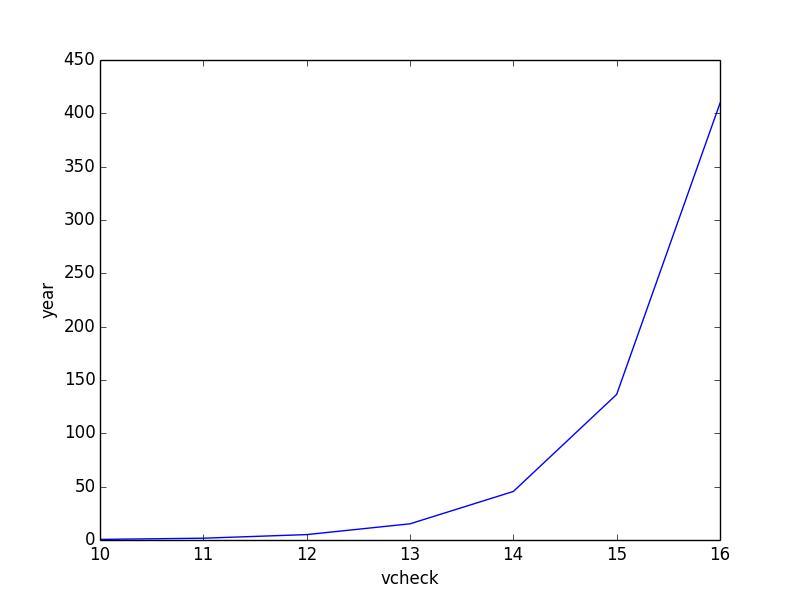
\includegraphics[width=10cm]{images/year.png}
	  \caption{It shows the waiting time for an adversary for a successful attack given that every parachain validators changes every 5 minutes}
	  \label{fig:totaltime}
\end{figure}

As it can be seen,  if $\totalchecks$ is more than 14, the adversary needs to wait more than 50 years for the attack. Therefore, in terms of security, it is important to have  minimum $\totalchecks$ validators.

\paragraph{The parameter $\mu$:} The possible $\mu$ (minimum number of extra check) values:

\begin{itemize}
    \item If $\mu = 0$, then $|pv| = 14$ in order to make sure that minimum $\totalchecks$ is always equal to $14$. Given that $|pv| = n/m$ where $m$ is the number of parachain validators $n = 14 * m$. 
    
    \item If $\mu > 0$, then $|pv| < 14$. It means that we need less validators for the security than in the case where $\mu = 0$. Less validators imply less network delay and less network delay implies more secure BABE. On the other hand, if $\mu$ increases, it means that more validators need to reconstruct a blob in order to check the validity. So, validators need to do more work. In terms of scalability of the relay chain, we need to decide $\mu$. 
\end{itemize}
As rule of thumb, if we don't care about the number of validators as far as it is not the maximum  number of validators ($N$) that Polkadot can handle, then if $14 * m < N$, $\mu = 0$. Otherwise, $\mu = 14 -N/m$. 

Another disadvantage of having $\mu = 0$ is that parachain validators have a less risky attack  when all of them are malicious. Imagine a parachain with a few collators. We can assume that they may be malicious and collaborate with the malicious validators. In this case, the validators will not have any report. So, there will be 0 extra checks. As soon as all parachain validators are malicious in this malicious parachain, they can add invalid block headers and cannot be caught. The security argument says here that they need to wait around 50 years for this, so the attack is not possible. However, in the real life, since the attack does not have any risk, the collators can bribe parachain validators with their stake and parachain validators validate an invalid blob.


Theorem \ref{thm:vcheckmal} gives the risk that  malicious validators take at  when they put an invalid report.  If $\mu + r \leq n/m$, the invalid block will not be detected with probability $\exp(-\frac{2}{3}(\mu+r))$. In the worst case scenario, if no report is received then the attack probability is $\exp(-\frac{2}{3}(\mu))$. We give in Figure \ref{fig:mu} that the probability of a successful attack in the case of $\totalchecks$ malicious validators are selected. As it can be seen in Figure \ref{fig:mu}, their risk is exponentially increasing when $\mu$ increases. In order to make the risk close to 0 even if no report received, $\mu$ should be greater than $4$.

\begin{figure}[h]\centering
	  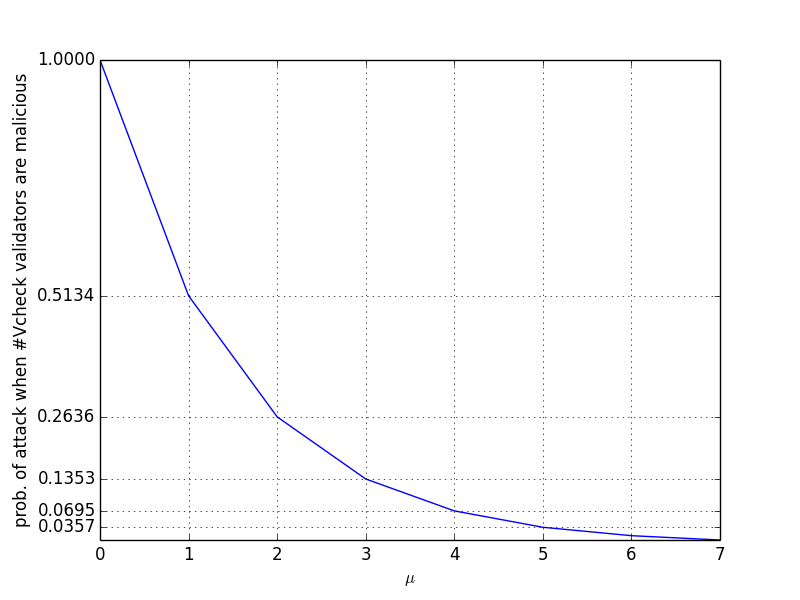
\includegraphics[width=12cm]{images/muval.png}
	  \caption{The risk of malicious validators when they attack even if $\totalchecks$ validators are malicious}
	  \label{fig:mu}
\end{figure}

\paragraph{Fisherman and Collator Reports:} In the validity scheme, we rely on the invalidity reports of fishermen and unavailability reports of collators to find the parameter $ \totalchecks $. However, we need to bound $\totalchecks$ so that these reports do not make too many validators check the validity. Let us call this bound $\mu_{max}$ (i.e, $\mu + \lceil r_f + r_a \rceil \leq \mu_{max}$). This bound is necessary because regular malicious reports can slow down the process easily. 

When a fisherman sends a report of invalidity, but later on it is found to be valid, the fisherman is slashed. Therefore, the reliability of a fisherman report can be measured by how much it is staked. 
Considering this, $r_f$ can be computed as follows:

$$r_f = \frac{\sum_{i}\mathsf{stake}_{f_i}}{v_{gain}}$$

Here, $\mathsf{stake}_{f_i}$ is the stake that a fisherman $f_i$ puts for this report and $v_{gain}$ is the DOT value that a validator receives in each block. In a nutshell, a fisherman needs to stake at least the same amount that the validator earns for each block in order to make a validator to execute an extra validity check. If the fisherman report is not valid, then the fisherman pays for this extra check. So, a malicious fisherman has to spend $\mu_{max} v_{gain}$ for a report to slow down the validator network. We believe that this model discourages fishermen from sending false reports. 

However, we cannot measure the reliability of unavailability reports as fisherman's reports since it is not possible to show the correctness or incorrectness of any unavailability reports. Malicious collators do not lose anything by just sending fake unavailability reports. In order to solve this issue, we assign a parameter $\alpha \in (0,1)$ for a parachain that defines the proportion of honest collator assumption. Depending on $\alpha$, we have defined $r_a$ for two cases:
\begin{itemize}
    \item if $\alpha > 1/2$, $r_a = \mu_{max}^{x/\alpha}$ 
    
        \[   
    r_a(x)= 
     \begin{cases}
       \mu_{max}^{x/\alpha} & \text{if } x \leq \alpha \\
       \mu_{max} &\text{otherwise} \\ 
     \end{cases}
\]  
    
    where 
    $$x = \frac{\text{total unavailability reports}}{\text{all collators}} = \frac{\sum_{c_i \in C_P}st_{c_i}}{|C_P|}.$$
    
    Here, $st_{c_i}\in \{0,1\}$ and it is 0 if the block is available. Otherwise, it is 1. The reason of using a function such as $\mu_{max}^{x/\alpha}$ is to make sure that we have extra checks close to maximum check only if the number of unavailability reports are close to the number of honest collator assumption. Thanks to this, if the number of honest collators are majority, the malicious collators who want to slow down Polkadot cannot achieve to make always maximum number of checks with only unavailability reports. In general, these type of parachains can be investigated by fishermen as far as the blocks are available to honest collators. Therefore, we expect that if there is any invalid block, the fishermen catch it and send a report. If the blocks are unavailable to honest collators (so fishermen too), validators check the invalidity with the maximum capacity.  
    
    \item if $\alpha < 1/2$, then it is critical to give more importance to the unavailability reports from this parachain. Therefore, we use the following linear function:
    
    \[   
    r_a(x)= 
     \begin{cases}
       \mu_{max}\frac{x}{\alpha} & \text{if } x \leq \alpha \\
       \mu_{max} &\text{otherwise} \\ 
     \end{cases}
\]  
\end{itemize}

So, $\mu' = \mu + \lceil r_a + r_f \rceil$ if $\mu + \lceil r_a + r_f \rceil \leq \mu_{max}$. Otherwise, $\mu' = \mu_{max}$.


\paragraph{The parameter $\mu_{max}$:} Given the fact that we have maximum number of extra checks when there are many invalidity or unavailability  reports, the parameter $\mu_{max}$ needs to be big enough so that the probability of having at least one honest extra check is almost 1.
This probability can be bounded by $1-(\frac{1}{3})^{\mu_{max}}$. Therefore, we can have $\mu_{max} = 15$.

In Figure \ref{fig:ra}, we compute the number of extra checks required depending on the $\alpha$-parameter of a parachain. As it can be seen, the parachain that we trust less requires more extra-checks. The parachain where we assume honest majority reaches the maximum check when the unavailability reports are close to the number of honest collators.  


\begin{figure}[h]\centering
	  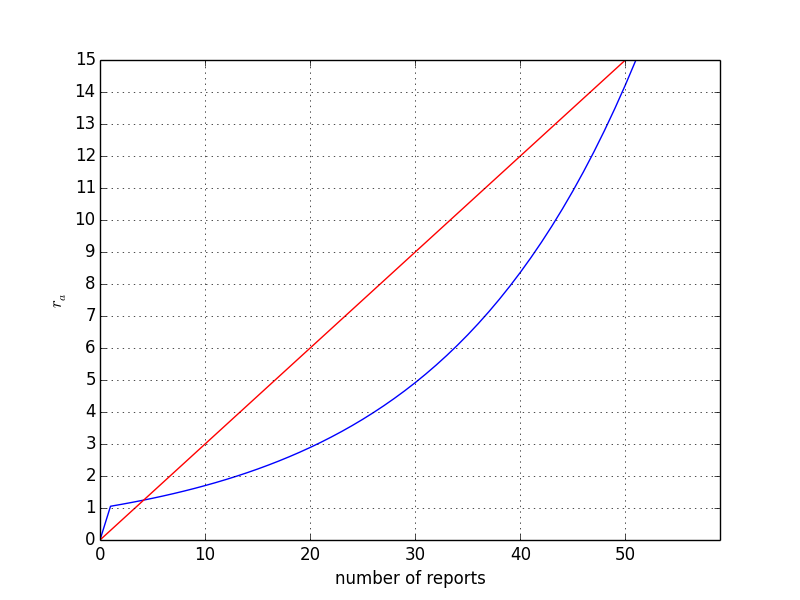
\includegraphics[width=10cm]{images/ra.png}
	  \caption{The red and blue graph shows the number of required extra checks when $\alpha \leq 1/2$ and $\alpha > 1/2$. Here, we assume that the total number of collators are 100.}
	  \label{fig:ra}
\end{figure}



\appendix
\section{Proof Details}

\newcommand\valord{\ensuremath{\mathcal{O}}}

\begin{lemma}\label{lem:permutation}
For any slot number $s$, block producer $bp$, epoch randomness $r$ for the epoch that includes $s$, integer $k >0$, and parachain $P$, with probability at least $1-(f/n)^{-k}$ over the epoch randomness and the random oracles for the hashes and VRFs, for any block that $bp$ produces in slot $s$ that includes a parachain header from $P$, if we eventually have $\totalchecks \geq k$ for this parachain header, then some honest validator checks the parachain block.
\end{lemma}
\begin{proof}
Consider generating an ordering $\valord$ of validators as follows, first we have the parachain validators in a uniformly random order, then all validators who satisfy condition (\ref{cond:mod}) (using $bp$'s VRF for slot $s$) in a uniformly random order, then we order all remaining validators in increasing order of the hash $H(ID_{PC} || \mathtt{VRF}_{\sk^v_j}(V))$ used in condition (\ref{cond:time}), breaking ties due to collisions in a uniformly random order. We claim that distribution of $\valord$ is as a uniformly random permutation of the validator set. To see this note that the only operation for which the different validators are treated differently are the VRFs and we assume that they are random oracles. The parachain validators are a set of $n/m$ validators chosen uniformly at random using $r$. Each validator satisfies condition (\ref{cond:mod}) with the same probability independently and so the distribution of the set of validators satisfying (1) conditioned on its size is a set of that size chosen uniformly at random from the non-parachain validators. Also the hashes in (2) are independently and identically distributed.

Next we show that for any block $bp$ produces in slot $s$ which includes a parachain header for $P$,  if any honest validator ever sees that $\totalchecks \geq k$, then any honest validators in the first $k$  validators in $\valord$ eventually check that block. All honest parachain validators and honest validators who satisfy (\ref{cond:mod}) check. If all honest validators in the fist $k$ validators in $\valord$ satisfy these conditions we are done. So suppose that $v$ is an honest validator in the first $k$ validators in $\valord$ who doesn't satisfy either of these conditions. $v$ will still check if $\tau$ is large enough and they don't see attestation from $\totalchecks$ validators who either are parachain validators, satisfied condition (\ref{cond:mod})  or had a smaller hash in condition (\ref{cond:time}). But noting that all such validators are before $v$ in $\valord$ so there can be at most $k-1$ of them. Thus $v$ only ever counts $k-1$ attestations towards the number needed $\totalchecks$ which is eventually $\geq k$. So when $\totalchecks \geq k$ and $\tau$ is large enough, $v$ checks.

Finally we need to show that the probability that the first $k$ validators in $\valord$ are honest is at least $(f/n)^k$. Since the first $k$ validators in $\valord$ are distributed as a set of $k$ validators chosen uniformly at random, this probability is $\prod_{i=0}^{k-1} (f-i)/(n-i) \leq (f/n)^k$.
\end{proof}

\end{document}
